\section{Interoperability}\label{section:interoperability2}

As introduced in Section~\ref{section:interoperability1}, \tool provides interoperability with existing e-learning applications based on the \gls{lti} standard. This section describes the concrete interoperability workflow.

\begin{figure}[t]
\centering
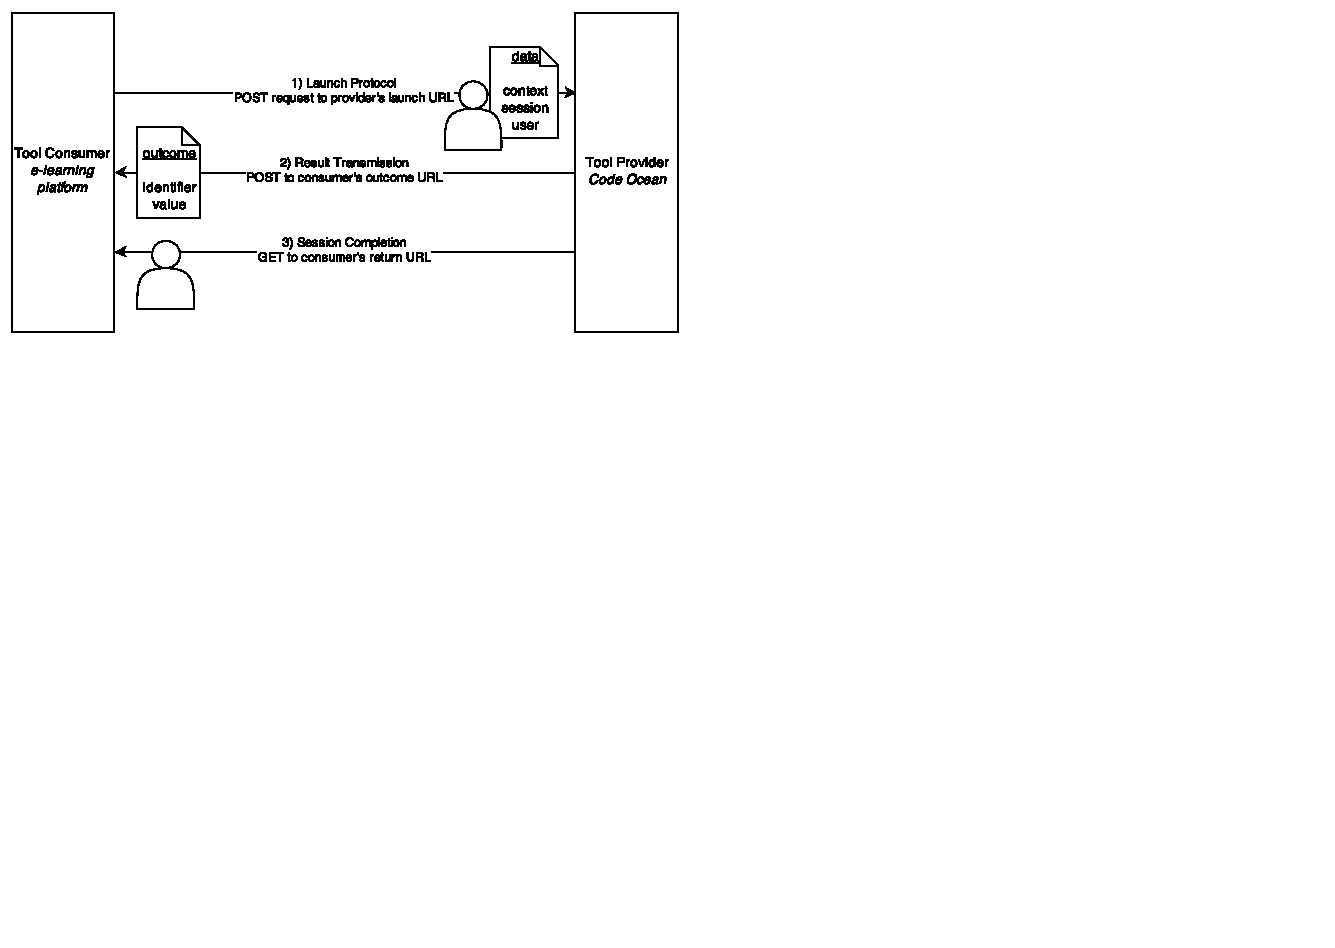
\includegraphics[clip=true, trim=0.1cm 10.3cm 11.1cm 0.2cm, width=\textwidth]{images/lti.pdf}
\caption{\gls{lti} Messages Exchanged in the Course of a Programming Session}
\label{figure:lti}
\end{figure}

As depicted in Figure~\ref{figure:lti}, a single programming session involves three different messages between a tool consumer and \tool. Initially, the tool consumer performs a launch request to start the programming session. Eventually, when the learner has finished her work, \tool transmits the learner's result to the consumer. Finally, the learner returns to the consumer application.

\subsection{Message Signing}

\Gls{lti} messages that are exchanged between a tool consumer and a tool provider are protected by means of OAuth 1.0\foo{http://oauth.net/core/1.0} message signing. This allows both parties to validate the integrity of received messages. Since message signing requires the exchange of credentials, consumer applications have to be registered with \tool and have to be provided with them. This way, only trusted consumer applications are able to profit from the services offered by \tool. The OAuth credentials comprise a client key and a shared secret. The client key uniquely identifies a consumer and is transmitted in plain text with every request. The shared secret is used for generating message signatures.

When a tool provider receives a signed \gls{http} request, it looks up the initiating tool consumer by means of the request's client key. Using the shared secret associated to this consumer, the provider can calculate the message signature in order to verify the message's integrity.

\subsection{Launch Protocol}

The launch protocol serves the purpose of sending a user from an e-learning application to a third-party application, such as a special-purpose tool. The protocol is based on a regular \gls{http} POST request sent from a tool consumer to a tool provider, which is either issued in a server-to-server fashion or, more commonly, through submitting an \gls{html} form on client side.

\subsubsection{Workflow}

In order to send a learner to \tool, a consumer application must perform a POST request towards \tool's \gls{lti} endpoint \gls{url}. Since \gls{lti} providers usually have a single endpoint, session-specific information is transmitted in the request's payload. To direct a learner to a specific exercise, \tool requires the exercise token (see Section~\ref{section:domain-model}) to be provided as a so-called custom parameter. Furthermore, an additional \emph{locale} parameter, which controls the \gls{ui}'s language, is supported.

If an incoming \gls{lti} launch request is validly signed, \tool creates an external user based on the provided information, signs her in, and redirects her to the specified exercise. In case of a prior visit by the same learner, no user is created, but the existing one is retrieved from the database.

\subsubsection{Launch Data}

Besides request metadata and OAuth attributes, the payload of a launch request contains a set of parameters that provide information specific to the guest user and the context from which the tool provider is accessed.

The \gls{lti} specification defines a double-digit number of supported parameters for the launch protocol. However, very few of these parameters are mandatory. Therefore, information provided by tool consumers can be greatly limited, for instance in case of strict privacy settings. The \gls{lti} standard specifies a set of recommended parameters and encourages tool consumers to provide as much data as possible. However, it also advises tool providers to tolerate missing information.

\begin{table}
\begin{tabular}{ l | c | l }
Name & Type & Value \\
\hline
custom\_locale & \emph{C} & de \\
custom\_token & \emph{C} & ff79903c \\
launch\_presentation\_return\_url & \emph{R} & http://example.org/lti/return \\
lis\_outcome\_service\_url & \emph{O} & http://example.org/lti/outcome \\
lis\_person\_contact\_email\_primary & \emph{R} & turing@example.org \\
lis\_person\_name\_family & \emph{R} & Turing \\
lis\_person\_name\_full & \emph{R} & Alan Mathison Turing \\
lis\_person\_name\_given & \emph{R} & Alan \\
lis\_result\_sourcedid & \emph{O} & c9a68d73f61bb832 \\
resource\_link\_id & \emph{M} & 42 \\
resource\_link\_title & \emph{R} & Fibonacci Sequence \\
roles & \emph{R} & Learner \\
user\_id & \emph{R} & 1912 \\
\end{tabular}
\caption{Exemplary \gls{lti} Launch Parameters}
\caption*{\emph{C}: custom parameter, \emph{M}: mandatory parameter, \emph{O}: optional parameter, \emph{R}: recommended parameter}
\label{table:lti-launch-parameters}
\end{table}

Table~\ref{table:lti-launch-parameters} presents a set of typical parameters for an exemplary launch request sent to \tool. Resource-specific parameters provide information regarding the link to access \tool from within the consumer application. User-specific information includes the student's email address, \gls{id}, name, and roles. The provided \gls{id} typically does not correspond to the consumer application's real user \gls{id}, but it is usually a uniquely generated key. The \emph{launch\_presentation\_return\_url} parameter represents the \gls{url} to redirect learners to as soon as the programming session is completed. The \emph{lis\_outcome\_service\_url} and \emph{lis\_result\_sourcedid} parameters indicate that the tool consumer accepts results and specify how to provide them. Finally, as mentioned above, the launch data contains custom parameters that are used to reference a specific exercise and to declare the learner's preferred locale.

The \gls{lti} standard specifies several user roles, including \emph{Administrator}, \emph{Instructor}, \emph{Learner}, and \emph{Staff}. However, since \tool uses \gls{lti} solely for providing learners access to the application, all external users are considered as such, regardless of the specified role.

\subsection{Result Transmission}

As covered in Section~\ref{section:assessment3}, when the student has finished her programming session and submits her code for terminal assessment, the final score is determined by executing the exercise's tests against the learner's solution.

If the tool consumer supports receiving results, the exercise score is normalized to a value between 0 and 1, as stipulated by the \gls{lti} standard, and sent to the outcome \gls{url} specified by the consumer. As discussed in Section~\ref{section:assessment2}, the responsibility to incorporate the practical assignment's score resides with the consumer application. In order to grant an appropriate score for finishing the assignment, the normalized score is usually multiplied by an assignment-dependent factor or used for a binary decision whether to award an adequate number of points.

Finally, the learner is signed out and redirected to a success page. This page contains her final score, a link to return to the consumer application, as well as some statistics regarding how well the learner performed in relation to her peers. Providing statistical information enables students to compare their scores with fellow students' ones and might be beneficial for long-term motivation~\cite{pieterse2013automated}.
